% Generated from 2026-EgoAnchor-Typst/egoanchor_cn_v4.typ.
% The LaTeX manuscript is the canonical source after this migration.
\documentclass[review]{vgtc}

\graphicspath{{figs/}{figures/}{pictures/}{images/}{./}}

% Keep the VR template's metrics and line spacing; only add Unicode/CJK fonts.
\usepackage{times}
\renewcommand*\ttdefault{txtt}
\usepackage{mathptmx}
\usepackage{fontspec}
\usepackage{xeCJK}
\setmainfont{Times New Roman}
\setsansfont{Arial}
\setmonofont{Courier New}
\setCJKmainfont[BoldFont=SimHei,ItalicFont=KaiTi]{SimSun}
\setCJKsansfont{Microsoft YaHei}
\setCJKmonofont{FangSong}

\usepackage{amsmath}
\usepackage{amssymb}
\usepackage{array}
\usepackage{booktabs}
\usepackage{multirow}
\usepackage{tabularx}
\usepackage{xcolor}

\onlineid{0}
\vgtccategory{Research}
\vgtcinsertpkg

\title{EgoAnchor：面向开放消费级混合现实的动态真实物体锚定}
\author{作者待定}
\authorfooter{}

\teaser{
  \centering
  \fbox{\rule{0pt}{2.0in}\rule{0.95\linewidth}{0pt}}
  \caption{EgoAnchor 系统概览。}
  \label{fig:teaser}
}

\abstract{%
动态真实物体锚定是透视混合现实（Passthrough Mixed Reality, PMR）中以真实物体为中心进行空间叠加的关键能力。现有方案通常依赖物理标记、专用传感器、平台级受限接口，或针对单个物体的离线准备流程，难以扩展到开放消费级场景中的日常刚性物体。本文提出 EgoAnchor，一套面向开放消费级混合现实的动态真实物体锚定系统。EgoAnchor 仅依赖头戴显示器双目图像与目标物体的可用三维模型，无需物理标记、专用深度硬件或逐物体离线训练，即可为日常刚性物体提供连续 6DoF 动态锚定能力。系统采用分层架构：视觉感知后端持续生成异步物体位姿流，对象锚定运行时则将其转换为世界坐标系下稳定、连续且可恢复的对象锚点。我们在 Meta Quest 3 上实现 EgoAnchor，并通过定量实验与用户研究评估其锚定精度、稳定性、响应行为和应用可用性。结果表明，EgoAnchor 能够在开放消费级 PMR 场景中稳定支持动态真实物体锚定。
}

\keywords{透视混合现实, 动态对象锚定, 6DoF 位姿估计, 动态物体追踪, 6D 物体定位}

\begin{document}

\firstsection{引言}\label{sec:introduction}
\maketitle

透视混合现实（Passthrough Mixed Reality, PMR）通过将虚拟内容实时叠加到真实环境，使用户能够直接围绕真实物体进行观察、操作与交互。近年来，随着 Meta Quest 3、Apple Vision Pro 等消费级头戴显示设备的普及，越来越多的混合现实应用开始围绕真实物体展开，例如虚拟说明书附着、物体高亮引导、桌面协同办公以及近物精细交互等。这类应用共同依赖一项基础能力：虚拟内容能够持续、稳定地附着于真实物体，并随物体运动保持一致的空间关系。

对于静态环境，这一目标通常可以通过空间锚点（Spatial Anchor）实现。然而，当用户拿起、移动、旋转或传递真实物体时，固定于环境中的空间锚点无法反映物体自身的运动，虚拟内容将随之产生明显偏移。因此，混合现实系统需要建立能够随真实物体运动持续更新的对象级空间参考，即动态对象锚定（Dynamic Object Anchoring）：无论用户自身运动、物体发生位姿变化，还是经历短暂遮挡，虚拟内容都应始终与真实物体保持稳定一致的六自由度（6DoF）对应关系。

现有系统已经从不同路径尝试支持对象级追踪与锚定。典型方案包括基于物理标签的跟踪、依赖深度或专用传感器的感知方法、平台提供的对象追踪接口，以及基于 CAD 或三维模型的商业对象识别框架。这些方法在受控环境中能够取得较好的效果，但仍难以同时满足开放消费级 PMR 场景的三个要求：第一，系统应具备开放性，能够在无需逐物体训练的前提下扩展到多类日常刚性物体；第二，系统应具备可部署性，能够在不依赖物理标签、专用深度硬件或受限平台接口的条件下运行于消费级头戴设备；第三，系统应提供稳定的动态对象锚定能力，即生成连续、世界一致且可恢复的 6DoF 对象锚点，而不仅仅是输出瞬时物体位姿。

实现这一目标需要同时解决两个问题。首先，系统必须将开放场景中的对象感知组织为可持续输出的异步物体位姿流，而不是一次性的检测或单帧位姿估计。其次，系统必须在设备持续运动、感知噪声、帧率不一致和短时目标丢失等实际运行条件下，将这些异步位姿估计转换为世界坐标系下稳定、连续且可恢复的对象锚点。前者决定系统能否面向开放日常物体进行感知，后者决定感知结果能否被 PMR 应用可靠地用于空间附着。

本文提出 EgoAnchor，一套面向开放消费级混合现实的动态真实物体锚定系统。EgoAnchor 采用对象感知与对象锚定解耦的分层架构，由视觉感知后端（Visual Perception Backend）和对象锚定运行时（Object Anchoring Runtime）组成。视觉感知后端基于头戴显示器双目图像与目标物体的可用三维模型，持续估计物体相对于设备的 6DoF 位姿，并输出异步物体位姿流。对象锚定运行时进一步将这些异步位姿转换到世界坐标系，并通过运行时转换策略生成可供 PMR 应用直接使用的对象锚点。整个系统无需物理标签、专用深度硬件或逐物体离线训练，可与现有三维模型资源以及近年来的 Image-to-3D 技术结合，为更多日常刚性物体提供部署潜力。

我们在 Meta Quest 3 上实现了 EgoAnchor，并通过定量实验和用户研究对系统进行了评估。定量实验利用官方控制器提供的高精度位姿作为参考，测量系统的锚定精度、稳定性与响应行为；用户研究围绕典型混合现实任务展开，评估系统在真实应用中的可用性。实验结果表明，EgoAnchor 能够在开放消费级 PMR 场景中稳定支持动态真实物体锚定。

本文的主要贡献如下：

\begin{enumerate}
  \item \textbf{EgoAnchor：} 一套面向开放消费级混合现实的动态真实物体锚定系统，仅依赖头戴显示器双目图像与目标物体的可用三维模型，即可为多类日常刚性物体提供连续 6DoF 动态锚定能力。
  \item \textbf{分层技术方案：} 一套由视觉感知后端与对象锚定运行时组成的分层技术方案。前者持续生成统一的异步物体位姿流；后者通过运行时转换策略，在设备持续运动、感知噪声和短时目标丢失等条件下，将异步物体位姿流持续转化为世界坐标系下稳定、连续且可恢复的对象锚点。
  \item \textbf{实现与评估：} 在 Meta Quest 3 上完成 EgoAnchor 系统实现，并通过定量实验与用户研究评估其在锚定精度、稳定性、响应行为和典型 PMR 应用任务中的可用性。
\end{enumerate}

\section{相关工作}\label{sec:related-work}


\subsection{平台级真实物体锚定}


真实物体锚定旨在为物理对象建立稳定的对象级空间参考，使虚拟内容能够持续附着于真实物体，是近年来混合现实平台的重要能力。随着消费级头戴显示设备的发展，主流 XR 平台逐步开始提供对象追踪或对象锚定能力，但在开放部署、对象泛化以及动态支持方面仍存在一定局限。

早期系统主要采用基于物理标记的方法，通过 AprilTag、ArUco 等人工标记获得稳定的位姿估计，ARToolKit、ARCore Augmented Images 等系统均属于这一范式。这类方法实现简单、鲁棒性较高，但需要预先在物体表面贴附标记，不仅改变真实物体外观，也难以适用于开放场景中的多类日常刚性物体。

近年来，消费级混合现实平台开始提供免标记对象追踪能力。HoloLens 2 的 Azure Object Anchors 利用设备感知与对象数字模型完成对象匹配，但公开资料显示其能力主要面向较大尺寸的静态对象；Apple Vision Pro 提供对象追踪能力，但依赖基于三维模型构建的参考对象以及离线训练流程；Vuforia Model Targets 基于对象形状以及三维模型实现真实物体识别与跟踪，但因其受约束的初始化与准备流程，常见于工业与设备场景；Meta Quest 近年来也开始支持动态对象追踪，但当前仍属于受系统支持对象集合与用户设置约束的受控能力。

总体而言，现有平台主要提供封装好的对象追踪能力，通常依赖专用硬件、受限的平台接口、模型准备或对象级离线流程，难以直接支持开放场景中的多类日常物体，也较少向开发者开放底层视觉感知结果。因此，开放消费级混合现实中的动态真实物体锚定仍然缺乏统一的系统支持。

\subsection{6DoF 物体位姿估计与跟踪}


6DoF 物体位姿估计旨在从图像中恢复刚性物体相对于相机的空间位姿，是动态真实物体锚定的感知基础。近年来，随着视觉基础模型的发展，相关研究不断降低对逐物体训练和专用硬件的依赖，使开放场景中的对象感知成为可能。

早期方法通常依赖局部几何特征与 PnP 求解，在弱纹理、遮挡以及复杂光照条件下鲁棒性有限。随后，大量深度学习方法针对特定物体学习位姿估计网络，如 PoseCNN、DenseFusion 等。进一步地，CosyPose、MegaPose 等方法结合渲染匹配提升了未知物体的泛化能力，FoundationPose 则实现了无需逐物体训练的零样本 6DoF 位姿估计。随着开放词表目标检测、视频对象分割、立体匹配等视觉基础模型的发展，开放场景中的对象感知能力得到进一步提升。然而，这些能力大多以独立视觉模块的形式存在，如何将其组织为面向混合现实应用的统一视觉感知流水线，仍然缺乏系统性的研究。

更重要的是，上述工作的目标始终是提升相机坐标系下 6DoF 位姿估计的准确性，而非混合现实中的对象锚定。视觉推理产生的异步时延、估计噪声以及跟踪波动，使高精度位姿流仍难以直接驱动稳定的虚实配准。换言之，现有研究主要关注对象感知，而如何将异步物体位姿流进一步转换为世界坐标系下稳定、连续且可恢复的对象锚点，仍然缺乏系统性的研究。

\subsection{XR 时延补偿与时间一致性}


配准误差（Registration Error）与端到端时延（End-to-end Latency）自增强现实诞生以来便被认为是影响用户体验的核心问题，也是导致虚实错位、视觉疲劳与沉浸感下降的重要原因。经典增强现实研究指出，时延与运动速度的乘积是动态配准误差的主要来源；后续系统分析进一步量化了不同误差源对配准精度的影响。对于依赖异步视觉感知的混合现实系统而言，图像采集、网络传输与模型推理通常会引入数十毫秒乃至更高的端到端时延；当物体或用户快速运动时，这种异步时延便会表现为虚拟内容相对于真实物体的明显漂移与打滑。

围绕时延补偿，学界与工业界发展出两类互补思路。其一是预测式跟踪：头部位姿外推可以降低动态配准误差，双指数平滑等方法提供了更轻量的预测替代。在交互输入侧，One Euro 滤波器以速度自适应的方式权衡抖动与延迟，是三维用户界面处理含噪输入的常用基线，但也揭示了卡尔曼滤波在快速运动下引入滞后的固有折衷。其二是后渲染对齐：后渲染三维 warp 将已渲染画面重投影到新视角，成为时间扭曲的概念源头；异步时间扭曲（ATW）在扫描输出前用最新头显位姿重投影画面，已成为消费级头显的标准时延补偿手段。

上述工作主要围绕头部运动预测、渲染重投影以及交互输入滤波展开，其目标是降低显示链路中的时延影响。相比之下，由异步视觉模块输出的对象位姿对应于历史采集时刻，其世界坐标关系需要结合设备历史位姿进行恢复。尽管 OpenXR 及各类平台运行时提供了设备级时空同步能力，这些机制主要面向设备自身位姿管理，尚未进一步支持由第三方异步视觉感知驱动的动态真实物体锚定。因此，如何面向异步物体位姿流建立统一的对象锚定运行时，仍然是消费级混合现实系统中的关键问题。

\section{方法}\label{sec:pipeline}


EgoAnchor 将动态真实物体锚定解耦为感知与锚定两层架构（如 \ref{fig:arch} 所示）。感知层负责\textbf{对象感知（Object Perception）}：从头戴显示器的双目图像与目标物体的先验三维模型中，持续恢复相机坐标系下的 6DoF 位姿估计，并输出即时可靠性评分，形成异步位姿流（Asynchronous Pose Stream）。锚定层负责\textbf{对象锚定（Object Anchoring）}：建立时空对齐机制与稳定化策略，将低频、含噪且伴随传输时延的异步位姿流转换为世界坐标系下连续、稳定且可恢复的对象锚点，直接驱动虚实配准。

\begin{figure*}[t]
  \centering
  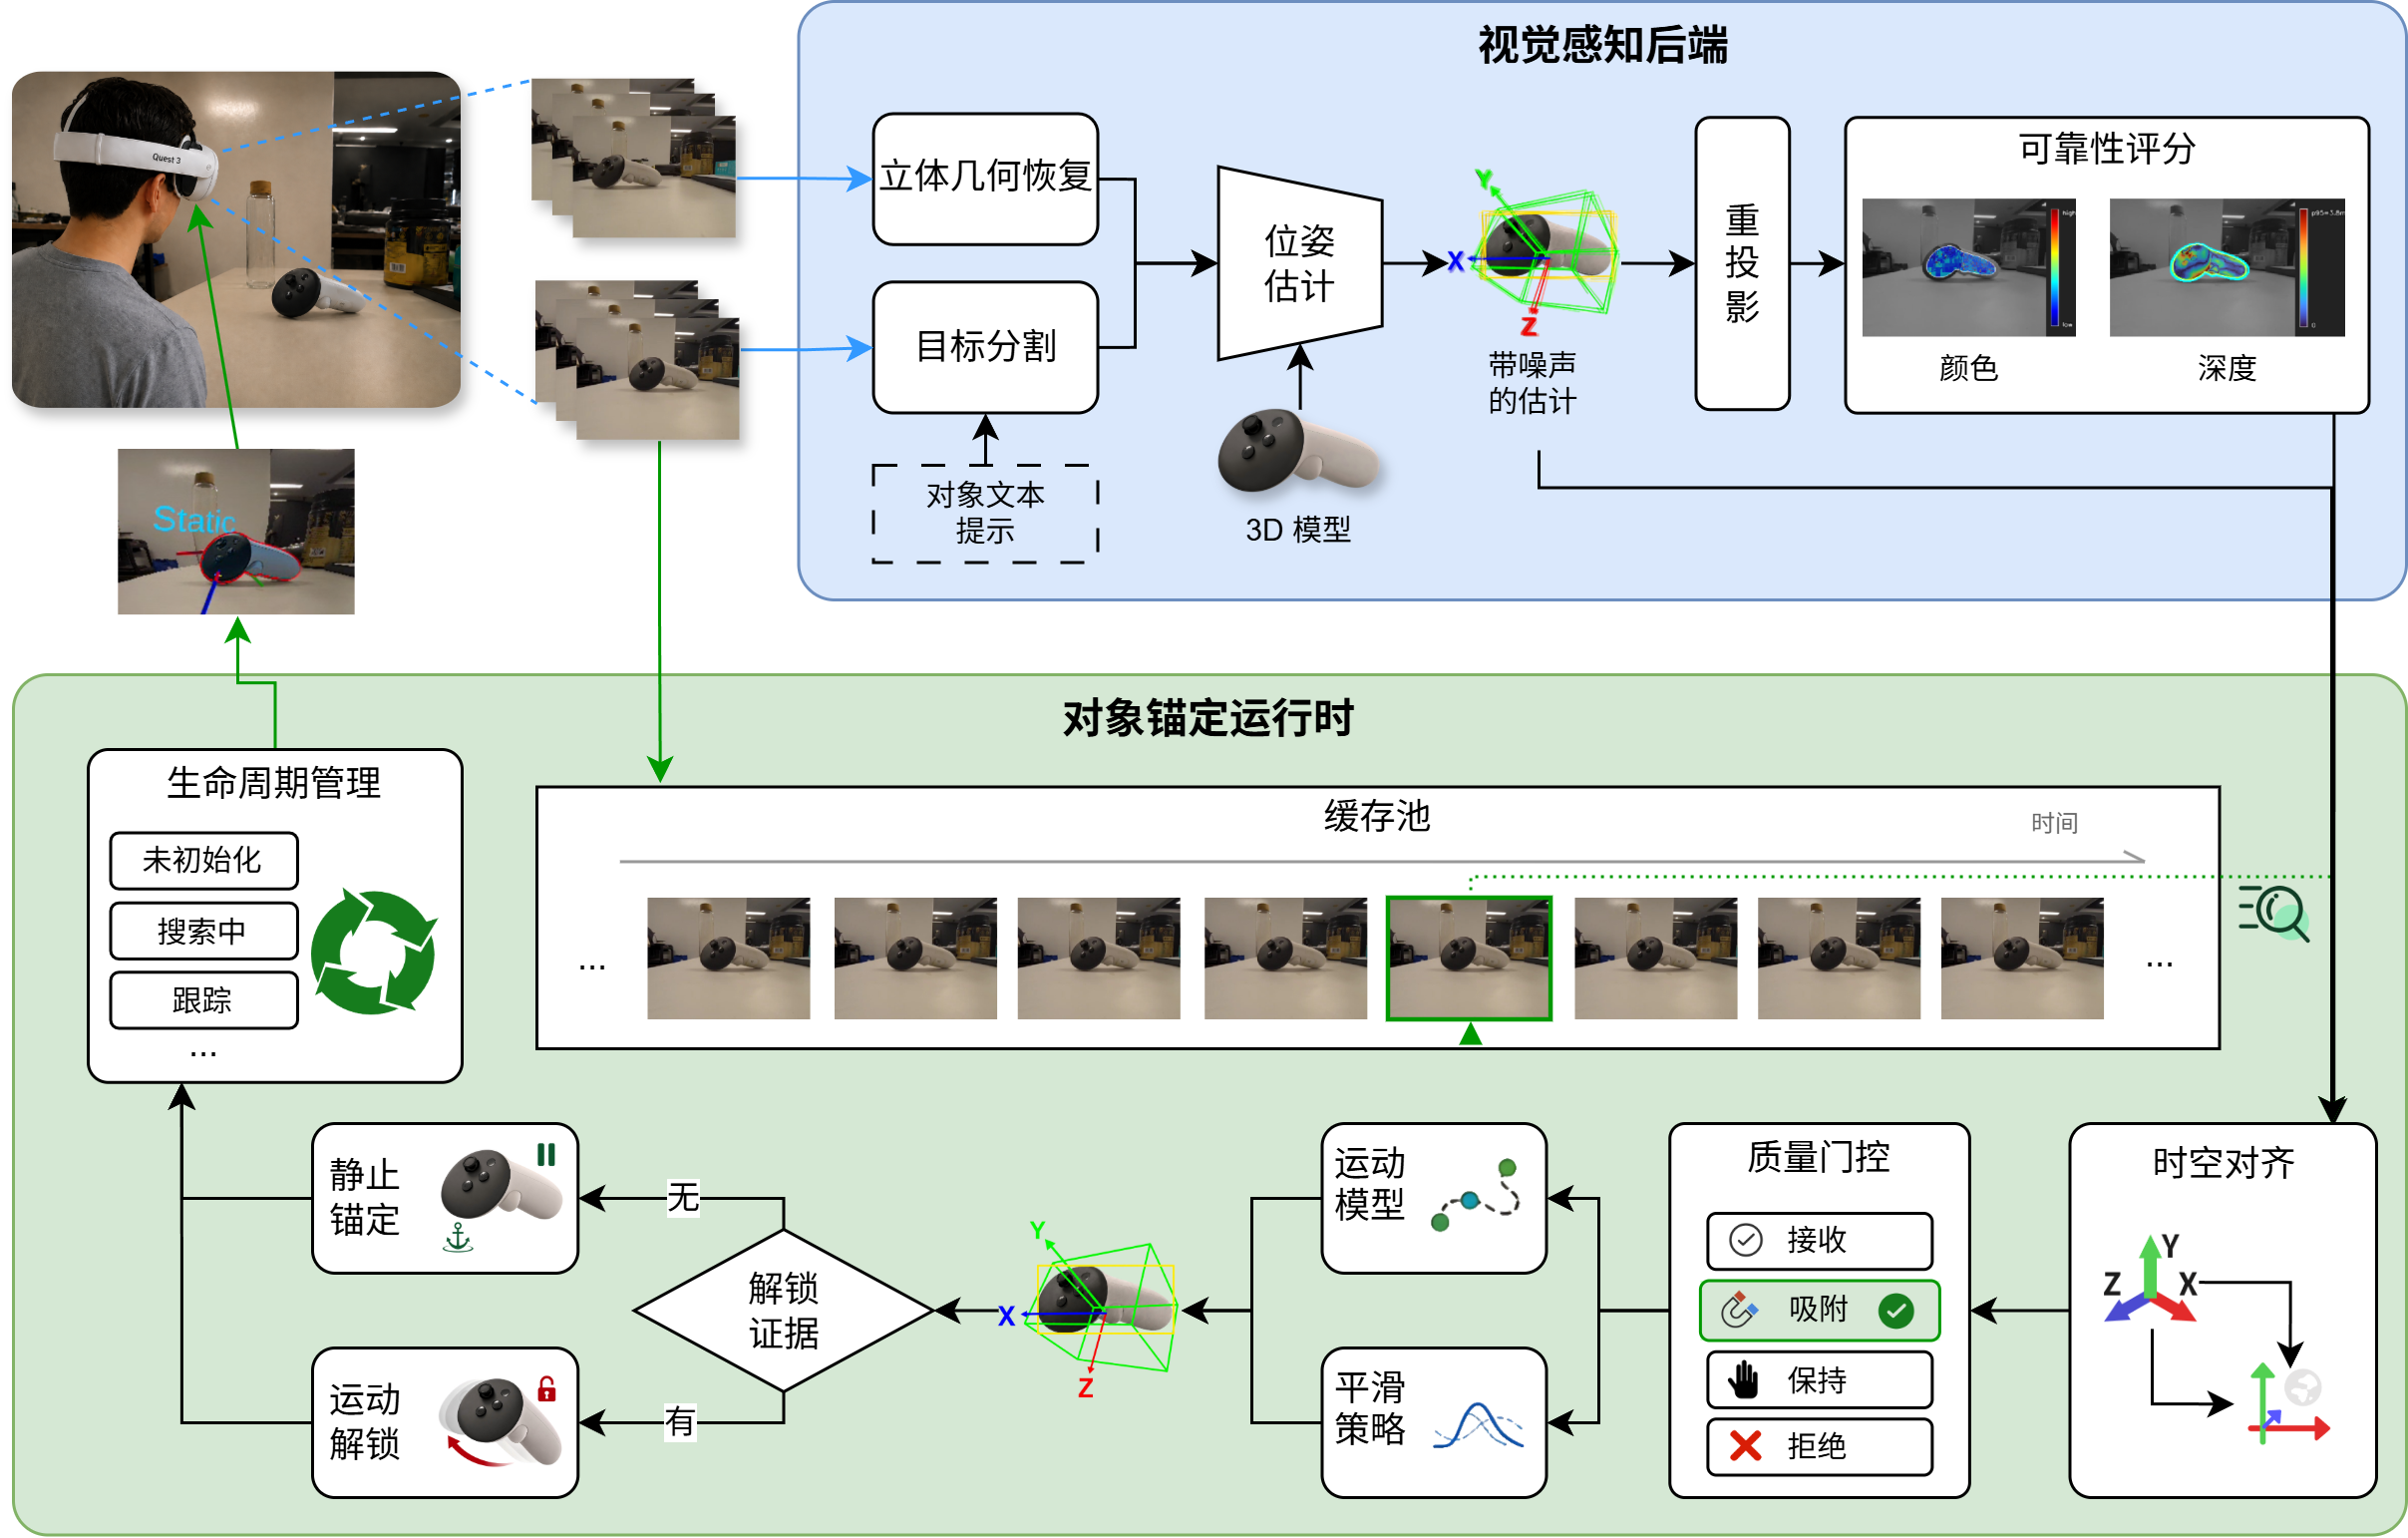
\includegraphics[width=0.95\textwidth]{figs/pipeline.png}
  \caption{EgoAnchor 分层架构。对象感知后端持续输出相机坐标系下的异步位姿流与可靠性评分；对象锚定运行时基于采集时刻的设备轨迹执行时空对齐，并通过双轴状态管理与多维稳定化策略合成世界坐标系下稳定、连续的对象锚点。}
  \label{fig:arch}
\end{figure*}


\subsection{对象感知}\label{sec:perception}


对象感知的数学目标是从双目图像帧对 $I_f = (I_f^L, I_f^R)$ 中持续恢复观测元组：

\begin{equation}
o_f = (T_o^{c_f}, R_f)
\label{eq:observation}
\end{equation}


其中，$T_o^{c_f} \in \mathrm{SE}(3)$ 为目标物体相对于相机坐标系的 6DoF 刚体位姿，$R_f \in [0,1]$ 为该观测的即时可靠性评分。观测序列 ${o_f}$ 构成异步位姿流，是连接对象感知与对象锚定的数据桥梁。

\subsubsection{零样本视觉推理}\label{sec:pipeline-detail}


实现开放场景下的对象感知需要同时满足两个约束：\textbf{零样本泛化性}------系统应能在无需逐物体训练的前提下扩展到多类日常刚性物体；\textbf{米制尺度一致性}------输出的位姿应具备绝对物理尺度，而非单目视觉中的尺度二义性。

EgoAnchor 采用多阶段视觉推理架构，通过协同四个关键模块构建统一的对象感知流水线：

\begin{enumerate}
  \item \textbf{目标语义分割（Target Semantic Segmentation）}：利用开放词表目标检测或多模态交互生成目标物体的初始语义掩膜 $M_0$，提供物体级的前景约束。
  \item \textbf{时序掩膜传播（Temporal Mask Propagation）}：通过半监督视频对象分割机制在连续帧间传播目标掩膜 $M_t$，在保证帧间一致性的同时显著降低逐帧分割的计算开销。
  \item \textbf{双目立体几何重建（Stereo Geometry Reconstruction）}：利用双目立体匹配从视差场恢复米制深度图 $D_t$，消除单目深度估计中固有的尺度二义性，为后续三维对齐提供绝对物理尺度基准。
  \item \textbf{零样本 6DoF 位姿估计（Zero-shot Pose Estimation）}：接收目标三维模型 $\mathcal{M}$ 与米制深度图 $D_t$；在初始化阶段结合语义掩膜 $M_0$ 执行全局注册，在时序追踪阶段以历史位姿为运动先验进行局部迭代优化，输出相机坐标系下的刚体位姿 $T_o^c \in \mathrm{SE}(3)$。
\end{enumerate}

对象感知流水线通过模块化组合实现零样本泛化：语义与时序模块提供稳定的前景分割，立体几何提供米制尺度约束，位姿估计完成三维对齐。对于追踪质量的评估与坏观测的过滤，系统依赖后续的可靠性感知评估机制统一处理。

\subsubsection{可靠性评分}\label{sec:reliability}


单帧位姿估计的几何输出无法直接量化其对虚实配准的可用性。感知算法可能在弱纹理、遮挡或光照变化下输出满足数学形式但物理错误的位姿。若被锚定运行时直接接受，将导致严重的虚实错位。因此，对象感知需要为每帧观测附加即时可靠性评分，以量化该观测对配准任务的可信度。

EgoAnchor 提出 VCD（Visibility-gated Color-Depth）可靠性评分模型。其核心思想是将当前位姿下的三维模型渲染回图像空间，通过比较渲染结果与实际观测的多模态一致性来验证位姿质量。该评分不用于评估 6DoF 算法本身的精度，而是作为运行时可靠性信号，用于在锚定运行时接收位姿前过滤明显错误的观测。评分公式为：

\begin{equation}
R = V \cdot G_{\mathrm{CD}}
\label{eq:reliability}
\end{equation}


其中 $R \in [0,1]$ 为最终可靠性评分。

\textbf{可视度因子} $V \in [0,1]$ 定义为观测掩膜与渲染投影掩膜的交集面积与渲染面积的比值：

\begin{equation}
V = (\lvert M_{\mathrm{obs}} \cap M_{\mathrm{rnd}} \rvert) / (\lvert M_{\mathrm{rnd}} \rvert)
\label{eq:visibility}
\end{equation}


其中 $M_{\mathrm{obs}}$ 为观测掩膜，$M_{\mathrm{rnd}}$ 为当前位姿下三维模型的渲染投影掩膜，$\lvert M \rvert$ 表示掩膜内像素数量。当物体部分遮挡、移出视野或当前位姿严重错位时 $V$ 下降，用于刻画目标的可见程度。

\textbf{几何一致性核} $G_{\mathrm{CD}} \in [0,1]$ 通过加权对数几何均值融合颜色投影相似度 $C$ 与深度几何对齐度 $D$：

\begin{equation}
G_{\mathrm{CD}} = \exp\!\left((w_C \ln \max\!\left(C, \epsilon\right) + w_D \ln \max\!\left(D, \epsilon\right)) / (w_C + w_D)\right)
\label{eq:cd-consistency}
\end{equation}


其中，权重设置为 $w_C = 0.2$、$w_D = 0.8$，几何下限 $\epsilon = 0.05$。相比线性加权，几何均值确保只有当颜色和深度证据均支持当前位姿时，才会获得高评分。深度通道权重更高是因为其直接度量三维几何一致性，而颜色受光照、反射等环境因素影响更大。几何下限的引入避免了极低分值在对数运算中导致的数值不稳定。

\textbf{颜色投影相似度} $C \in [0,1]$ 度量渲染与观测图像的颜色一致性。为避免边缘配准误差与高光反射的影响，在渲染投影与观测掩膜交集的内部区域，采用 CIELAB 色彩空间计算零均值归一化互相关（ZNCC）：

\begin{equation}
\mathrm{ZNCC} = (\sum_{p} \mathbf{w} \cdot (\widetilde{\mathbf{I}}_{\mathrm{rnd}}^p) \cdot (\widetilde{\mathbf{I}}_{\mathrm{obs}}^p)) / (\sqrt{\sum_{p} \lVert \mathbf{w} \cdot \widetilde{\mathbf{I}}_{\mathrm{rnd}}^p \rVert^2} \sqrt{\sum_{p} \lVert \mathbf{w} \cdot \widetilde{\mathbf{I}}_{\mathrm{obs}}^p \rVert^2})
\label{eq:zncc}
\end{equation}


其中 $\widetilde{\mathbf{I}}^p = \mathbf{I}^p - \mathbf{\mu}$ 为去均值后的 LAB 三通道向量，$\mathbf{w} = [w_L, 1, 1]^T$ 为通道权重向量，$w_L = 0.3$ 降低亮度通道权重以减弱对光照变化的敏感性。ZNCC $\in [-1,1]$ 通过线性映射归一化到颜色相似度：

\begin{equation}
C = (1 + \mathrm{ZNCC}) / 2
\label{eq:color-sim}
\end{equation}


颜色一致性作为辅助证据，对纹理明显的物体有帮助，但在纯色或无纹理物体上，该项会被自动排除而不会惩罚评分。

\textbf{深度几何对齐度} $D \in [0,1]$ 度量观测深度与渲染深度的空间一致性。双目立体深度在高频几何表面易产生系统性偏差，单纯的逐像素残差统计难以区分"深度形状正确但有全局偏移"和"位姿真正错误"。系统采用绝对残差 $D_{\mathrm{abs}}$ 与相对结构 $D_{\mathrm{struct}}$ 的联合评估：

\begin{equation}
D = (1-\alpha) D_{\mathrm{abs}} + \alpha D_{\mathrm{struct}}
\label{eq:depth-joint}
\end{equation}


绝对残差分量 $D_{\mathrm{abs}}$ 度量逐像素深度差异的统计分布。在核心区域（轻量腐蚀 mask 以排除边缘噪声）内，采用距离自适应容差联合评估内点比例与归一化残差中位数：

\begin{equation}
\tau(p) = \max\!\left(\tau_{\mathrm{min}}, \rho_z D_{\mathrm{rnd}}(p)\right)
\label{eq:depth-thresh}
\end{equation}


\begin{equation}
D_{\mathrm{abs}} = \lambda \rho_{\mathrm{inlier}} + (1-\lambda) S_{\mathrm{med}}
\label{eq:depth-abs}
\end{equation}


其中内点比例与归一化残差中位数定义为：

\begin{equation}
\rho_{\mathrm{inlier}} = 1/(\lvert \Omega \rvert) \sum_{p \in \Omega} \mathbf{1}[e(p) < \tau(p)]
\end{equation}


\begin{equation}
S_{\mathrm{med}} = 1 - \mathrm{median}_{p \in \Omega} (\min\!\left(e(p)/(s \cdot \tau(p)), 1\right))
\label{eq:depth-stats}
\end{equation}


参数设置为 $\tau_{\mathrm{min}} = 5 \mathrm{mm}$（对应Quest双目深度噪声地板）、$\rho_z = 0.02$（2\%的距离比例）、$\lambda = 0.6$（更重视覆盖率）、$s = 2.5$（鲁棒应对系统性偏差的残差容忍倍数）。

相对结构分量 $D_{\mathrm{struct}}$ 通过归一化深度的零均值互相关（ZNCC）评估深度波峰波谷的空间对应关系。对渲染深度和观测深度分别减去各自中位数并除以四分位距（IQR）归一化后，按公式 \ref{eq:zncc} 计算ZNCC并映射到 $[0,1]$ 区间。该方法使系统能够识别深度形状完全对齐的正确位姿，即使存在全局偏移或局部系统噪声。

融合权重 $\alpha$ 根据场景复杂度自适应调整：

\begin{equation}
\alpha = \begin{cases}
0, & \mathrm{IQR} < \tau_{\mathrm{IQR}}, \\
\alpha_{\mathrm{max}} \cdot \min\!\left(\mathrm{IQR}/\tau_{\mathrm{IQR}}, 1\right), & \mathrm{IQR} \geq \tau_{\mathrm{IQR}}
\end{cases}
\label{eq:depth-alpha}
\end{equation}


其中 $\alpha_{\mathrm{max}} = 0.35$，$\tau_{\mathrm{IQR}} = 20 \mathrm{mm}$。平坦表面时完全回退到绝对残差评估，高频几何时引入结构验证以区分系统噪声与真正错位。

\subsection{对象锚定}\label{sec:anchoring}


对象锚定的核心任务是建立从相机坐标系异步位姿流到世界坐标系对象锚点的稳定映射。这一过程需要同时解决三个挑战：\textbf{一致性}------将历史时刻计算的相机系位姿正确转换到世界坐标系；\textbf{稳定性}------在感知噪声与用户头动下保持虚实配准稳定；\textbf{连续性}------在目标短暂遮挡或追踪失效后快速恢复锚定。

\subsubsection{时空对齐}\label{sec:alignment}


异步视觉推理产生的观测到达运行时时已滞后于采集时刻。若使用到达时刻的设备位姿变换历史观测，将引入与设备运动速度线性相关的动态配准误差。运行时在图像采集时将帧标识 $f$ 与相机世界变换 $T_c^w(f)$ 写入有界缓存；观测 $o_f$ 到达时，通过 $f$ 检索采集时刻的设备位姿，合成世界坐标系下的目标位姿：

\begin{equation}
T_o^w (f) = T_c^w (f) \circ T_o^{c_f}
\label{eq:world-transform}
\end{equation}


其中 $\circ$ 表示刚体变换的复合。这一时间对齐机制将动态配准误差降低到仅受感知算法自身精度约束。

除时间对齐外，运行时还需执行空间坐标系对齐。视觉感知后端基于 OpenCV 约定输出位姿（右手系，$+X$ 向右、$+Y$ 向下、$+Z$ 向前），而混合现实运行时采用 Unity 世界坐标系（左手系，$+X$ 向右、$+Y$ 向上、$+Z$ 向前）。系统在应用公式 \ref{eq:world-transform} 前，通过坐标系转换矩阵 $T_{\mathrm{Unity}}^{\mathrm{OpenCV}}$ 将观测位姿从视觉坐标系变换到渲染坐标系。该矩阵对应沿 $X$ 轴的 $\pi$ 旋转，同时完成从右手系到左手系的手性变换。时间对齐消除异步时延引入的动态误差，空间对齐确保几何一致性，二者共同保证异步视觉观测被正确映射到混合现实世界参考系。

\subsubsection{运动估计与平滑}\label{sec:smoothing}


世界坐标系下的观测序列 ${T_o^w (f)}$ 仍受视觉位姿估计不确定性与跨端传输时延波动影响。一方面，零样本位姿估计算法在光照变化、遮挡与弱纹理等条件下产生的位姿估计存在逐帧波动；另一方面，感知后端到锚定运行时的网络传输引入的时延抖动使观测到达间隔不均匀。运行时需将这种低频、含噪且时序不规则的观测流转换为高帧率稳定轨迹。系统采用运动估计与时序平滑的两阶段策略：前者从观测中恢复状态与速度，后者将状态合成为渲染输出。

运动估计采用常速度卡尔曼滤波。状态向量 $\mathbf{x} = [\mathbf{p}, \mathbf{v}]^T$ 联合编码位置 $\mathbf{p} \in \mathbb{R}^3$ 与速度 $\mathbf{v} \in \mathbb{R}^3$，通过预测-更新循环实现位置与速度的联合估计。位置通道与旋转通道分别维护独立的状态估计器，旋转通道在对数映射空间执行相同的常速度滤波。

时序平滑采用延迟插值策略。系统根据实测采集-渲染延迟自适应引入延迟 $\Delta$（实测延迟 $\times$ 安全系数，典型值 100--350 ms），使渲染时刻 $t$ 的输出锚点取在历史时刻 $t - \Delta$ 处。由于 $t - \Delta$ 落在已到达的卡尔曼滤波控制点 ${(t_k, \mathbf{p}_k, \mathbf{v}_k)}$ 之间，输出为插值而非外推，从而避免了预测外推引入的不确定性。位置与旋转通道分别采用 Hermite 样条插值，以控制点处的速度 $\mathbf{v}_k$ 作为端点切线 $\mathbf{m}_k$，确保插值曲线在控制点处与速度估计一致。

为避免物体急停时速度估计滞后导致的过冲振铃，系统通过 Fritsch-Carlson 单调性约束限制切线模长。设第 $k$ 个控制点位于 $t_k$，对应位置 $\mathbf{p}_k$ 与切线 $\mathbf{m}_k$，相邻控制点间的时间间隔为 $\Delta t_k = t_{k+1} - t_k$，则切线模长被钳制为：

\begin{equation}
\lVert \mathbf{m}_k \rVert_2 \leq \kappa (\lVert \mathbf{p}_{k+1} - \mathbf{p}_k \rVert_2) / (\Delta t_k)
\label{eq:tangent-clamp}
\end{equation}


其中 $\kappa = 3$ 为单调性系数。当相邻控制点间的位移弦长 $\lVert \mathbf{p}_{k+1} - \mathbf{p}_k \rVert_2$ 趋近于零时（物体减速或停止），切线被自适应压缩，防止插值曲线超出控制点包络。该策略将低频观测平滑为连续轨迹，为后续稳定化提供基线输出。

\subsubsection{静止锚定}\label{sec:staticlock}


运动估计与平滑策略将低频观测转换为连续轨迹，但无法消除静止期的高频抖动。传统滤波器通过增大平滑系数可抑制抖动，但代价是引入运动滞后，这一权衡源于其运动无关（Motion-agnostic）特性------无法区分静止期噪声与真实运动初始加速。

EgoAnchor 通过\textbf{静止锚定（Static Anchoring）}打破这一权衡：显式建模静止状态，在静止期冻结输出锚点，在运动期交回平滑输出。当物体速度与可靠性评分在驻留窗口 $t_{\mathrm{dwell}}$（典型值 350 ms）内持续满足锁定条件时，系统激活静止锁：

\begin{equation}
\lVert \mathbf{v} \rVert_2 \leq v_{\mathrm{th}}, \quad \lVert \mathbf{\omega} \rVert_2 \leq \omega_{\mathrm{th}}, \quad R \geq R_{\mathrm{min}}
\label{eq:lock-condition}
\end{equation}


其中 $\mathbf{v} \in \mathbb{R}^3$ 与 $\mathbf{\omega} \in \mathbb{R}^3$ 分别为估计的线速度与角速度，$v_{\mathrm{th}}$（典型值 5 cm/s）与 $\omega_{\mathrm{th}}$（典型值 22°/s）为静止判定的速度阈值，$R_{\mathrm{min}}$（典型值 0.25）为最低可靠性要求。角速度阈值设为观测噪声地板的约 1.5 倍，在抑制噪声波动与快速进入锁定之间取得平衡。锁定后，输出冻结于锁定原点 $T_L$（由锁定前观测的指数移动平均确定），实现静止期的稳定输出。

进入锁定后，系统并行运行四路独立的解锁判定通道，任一通道触发则立即解锁：

\textbf{速度逃逸}：观测速度明确超出静止阈值的显著倍数（$\gamma_v = 2.5$）且持续超过抗噪声窗口（50 ms）时立即解锁，应对用户拿起或挥动物体的高速突发运动。

\textbf{漂移阻缰}：系统维护观测共识 $T_{\mathrm{cons}}$（被接受观测的低增益指数移动平均），监测其相对锁定原点的累积空间距离。一旦位移超出阻缰阈值 $d_{\mathrm{tether}}$（典型值 1.5 cm）或旋转超出 $\theta_{\mathrm{tether}}$（典型值 5°），强制解锁以防止慢速但持续的大位移运动被噪声容差吞噬。速度逃逸与漂移阻缰互补：前者响应高速突发运动（如用户拿起物体），后者防止慢速平移累积（如物体在桌上缓慢滑动）。

\textbf{可靠性加权累积和}：在噪声容差 $\delta$（典型值 8 mm）外，通过带遗忘因子的累积和积分超出容差的位移证据：

\begin{equation}
U_k = \lambda^{(\Delta t_k) / \tau} U_{k-1} + ((\Delta t_k) / (\Delta t_0)) R_k \max\!\left(0, \lVert \mathbf{p}_k - \mathbf{p}_L \rVert_2 - \delta\right)
\label{eq:cusum}
\end{equation}


其中 $\mathbf{p}_k$ 为第 $k$ 次观测的位置，$\mathbf{p}_L$ 为锁定原点位置，$\Delta t_k$ 为距上次观测的时间间隔，$\Delta t_0 = 16.7$ ms 为归一化基准，$\lambda = 0.5$ 为遗忘因子，$\tau = 500$ ms 为时间常数。当 $U_k$ 超过解锁阈值 $U_{\mathrm{th}}$（典型值 8 cm）时触发解锁。该机制通过时间累积将多次微小但一致的位移累加为解锁证据，应对容差内的细微持续运动。可靠性加权 $R_k$ 确保低分观测的贡献被抑制，防止感知质量下降时的误解锁。

\textbf{低分释放}：可靠性评分持续低于极低阈值 $R_{\mathrm{release}}$（典型值 0.3）超过时间窗口（600 ms）时主动解锁。当物体被移出视野或严重遮挡时，继续冻结输出将导致锚点停留在错误位姿，低分释放确保系统在感知失效时交回控制权，配合上层的重获取机制重建追踪。

为应对头部运动引起的视觉滑移与测量距离相关的深度噪声，系统对判定阈值进行自适应调整。首先，根据头显线速度 $\lVert \mathbf{v}_{\mathrm{head}} \rVert_2$ 与角速度 $\lVert \mathbf{\omega}_{\mathrm{head}} \rVert_2$ 自适应放大静止判定阈值 $v_{\mathrm{th}}$ 与噪声容差 $\delta$，放大系数与头部速度成比例；当头部停止后进入沉降期 $t_{\mathrm{settle}}$（典型值 600 ms），冻结所有解锁判定以消化残留重投影误差。其次，根据物体到头部的欧氏距离 $z$ 自适应缩放位置通道容差，以补偿立体深度不确定性随距离二次方增长的特性：

\begin{equation}
\delta'(z) = \delta \cdot \min\!\left(f_{\mathrm{max}}, 1 + \gamma_z (z - z_{\mathrm{ref}}) / z_{\mathrm{ref}}\right)
\label{eq:distance-adaptive}
\end{equation}


其中 $z_{\mathrm{ref}} = 40$ cm 为参考距离，$\gamma_z = 1.0$ 为距离放大系数，$f_{\mathrm{max}} = 3.0$ 为最大放大倍数。

解锁瞬间，系统以指数衰减方式将锁定位姿与平滑输出的残差融合，确保连续过渡。静止锚定通过显式建模静止状态，在静止期实现高稳定性输出，通过多通道并行检测与可靠性加权，在运动响应性上与滤波基线相当。

\subsubsection{生命周期管理}\label{sec:lifecycle}


对象锚点的持续可用性依赖于跨越初始化、追踪维护、短暂丢失与恢复的完整生命周期管理。运行时通过状态机协调感知质量监测与锚定策略切换，确保锚点在目标可观测时保持稳定追踪，在感知失效时平滑退化并自动恢复。

系统启动后，感知后端通过开放词表目标检测（基于 YOLO-World）自动识别场景中的目标物体类别并执行语义分割，生成初始目标掩膜。锚点进入搜索状态，感知后端执行全局位姿注册（见 \ref{sec:pipeline-detail}）。首次观测可靠性评分 $R$ 超过初始化阈值后，锚点转入追踪状态，开始接收异步观测并应用 \ref{sec:alignment} -- \ref{sec:staticlock} 描述的对齐、平滑与稳定化策略。

追踪期间，运行时持续监测距离最近一次可靠观测的时间间隔。若可靠性评分持续低于维持阈值，系统停止接受新观测，根据时间间隔长度进入相应的退化状态：在短时间内（典型值 450 ms 以内），锚点进入滑行状态，输出由 \ref{sec:smoothing} 的平滑策略维持------在延迟插值窗口内通过已有控制点插值生成，超出窗口时退化为基于最后已知状态的短时外推；若时间间隔进一步增长但仍在可接受范围内（典型值 1 s 以内），锚点转入冻结状态，保持最后已知位姿但标记为不确定；若时间间隔超过上限，锚点标记为丢失。

在滑行、冻结或丢失状态下，若感知后端恢复高质量观测（评分超过恢复阈值且持续稳定），运行时自动将锚点与当前观测重新关联，恢复追踪状态。这一自动重获取机制使锚点在感知质量波动时保持鲁棒：短暂遮挡通过滑行平滑度过，中等时长丢失进入冻结保护，持续丢失则触发完整恢复流程，避免错误观测破坏已建立的空间参考。

\section{系统实现}\label{sec:impl}


我们在 Meta Quest 3 上实现 EgoAnchor，采用客户端-服务端分离架构。视觉感知后端运行于搭载 NVIDIA RTX 3090 GPU 的桌面计算设备（Windows 11，Intel Core i9-14900K，32 GB 内存），基于 Python 3.12、PyTorch 2.7、CUDA 12.8 实现，通过 Wi-Fi 6 与头戴设备连接；对象锚定运行时与渲染应用以原生方式运行于头戴设备，基于 Unity 6 (6000.3.11f1) 与 Meta XR SDK 203.0 实现。Quest 3 通过 Passthrough Camera API 提供双目图像流，相机内参与分辨率由运行时动态读取。

\subsection{视觉感知后端}


感知后端按 \ref{sec:pipeline-detail} 描述的流程实现零样本视觉推理。目标语义分割采用 YOLOE26 结合 SAM3 生成初始掩膜，时序传播通过 Cutie 实现，双目深度估计采用 Fast-FoundationStereo 并通过 TensorRT 加速（FP16 精度），6DoF 位姿估计采用 FoundationPose（初始注册迭代 5 次、跟踪迭代 2 次）。可靠性评分模块（\ref{sec:reliability}）通过 nvdiffrast 实现可微渲染，生成颜色图、深度图与投影掩膜，计算 VCD 综合评分。流水线采用异步编排，语义分割、立体匹配与掩膜传播并行执行，通过 CUDA 流隔离与无锁队列解耦各阶段。

在 RTX 3090 平台上，完整的视觉推理流水线平均每帧耗时约 140 ms（约 7 fps）。为评估系统在不同算力条件下的性能表现，我们在 RTX 4090 与 RTX 5090 平台上进行了对照测试：RTX 4090 平台的平均推理时间降至约 100 ms（约 10 fps），RTX 5090 平台进一步降至约 65 ms（约 15 fps）。

\subsection{对象锚定运行时}


锚定运行时以 C\# 实现，基于 Meta XR SDK 的 \texttt{PassthroughCameraAccess API} 获取双目图像与相机内参。运行时维护容量为 512 项的环形缓冲区存储设备历史位姿，通过帧标识 $f$ 精确回查采集时刻的相机世界变换 $T_c^w (f)$，按 \ref{eq:world-transform} 合成世界坐标系下的对象锚点。

运动估计采用常速度卡尔曼滤波，位置与旋转通道分别维护独立滤波器，观测噪声协方差根据可靠性评分 $R$ 自适应调整。时序平滑采用延迟插值策略，主动引入固定延迟（典型值 120 ms），通过 Hermite 样条在已到控制点间插值。静止锚定通过状态机实现（\ref{sec:staticlock}），在串流模式下以约 60 Hz 频率更新锚定判定与四路解锁证据，头部速度与物体距离用于自适应调整容差。

\subsection{跨端通信}


系统采用双平面传输架构。数据面通过 ZeroMQ 的发布-订阅模式传输双目 JPEG 图像流（端口 15557），订阅端配置激进的最新帧保留策略，仅保留最新帧以匹配实时追踪需求。消息面通过 NATS 传输位姿结果、状态事件与控制命令（端口 4222），采用 Protobuf 序列化，命令通过请求-应答模式实现幂等执行。

帧标识 $f$ 作为跨端对齐主键，贯穿图像采集、位姿估计与锚点合成全流程；时间戳仅用于端到端时延诊断，不参与位姿计算。

\section{评估}\label{sec:eval}


\subsection{实验设置}


我们在 Meta Quest 3 上评估 EgoAnchor，采用两条互补的评估轨道。第一条为定量轨：以 Meta Quest 官方控制器作为评估目标，其六自由度位姿由平台软件开发工具包直接给出，可作为高精度真值，用于精确度量锚定精度、稳定性与响应行为；由于控制器与头显共享同一追踪系统，该真值能够隔离视觉位姿到锚点的转换栈，无需额外的物体到真值外参标定。第二条为应用轨：在多类日常刚性物体上开展用户研究，并辅以无需真值的客观代理指标，评估系统在真实任务中的可用性与对开放物体的泛化能力。两条轨道分别支撑下文的定量评估（RQ1、RQ2）与应用评估（RQ3）。评估全程记录视觉感知后端与对象锚定运行时两端的日志，并依据帧标识与共享会话标识自动配对，供离线分析使用。

\subsection{研究问题}


评估围绕三个研究问题展开，分别从锚定质量、设计权衡与泛化能力三个维度验证系统的有效性。

\textbf{RQ1：锚定质量（Anchoring Quality）} --- EgoAnchor 能否在开放消费级 PMR 场景中实现满足应用需求的动态对象锚定？具体在精度、稳定性、响应性和鲁棒性维度表现如何？

\textbf{RQ2：设计权衡（Design Trade-offs）} --- 分层架构与静止锚定在稳定性与响应性之间取得了怎样的权衡？相对于运动无关的平滑方法有何优势？

\textbf{RQ3：泛化能力（Generalization）} --- EgoAnchor 在多类日常刚性物体与典型应用场景中的泛化能力如何？系统的适用边界在哪里？

运动估计与时序平滑的具体选择是可替换的实现细节，其设计空间对比置于补充材料。时空对齐与静止锚定是系统的核心设计选择，我们通过消融研究验证其贡献。

\subsection{定量评估}


\subsubsection{评估指标}


定量评估在控制器目标上进行，从录制日志中计算一组锚定体验质量指标：

\begin{itemize}
  \item \textbf{锚定误差}：锚点与真值之间的相对位姿误差，分别报告平移（mm）与旋转（度）分量，刻画系统的绝对精度。
  \item \textbf{静止期抖动}：真值静止窗口内经高通滤波后的位置与旋转均方根，度量静止稳定性。
  \item \textbf{运动滞后}：锚点速度与真值速度的互相关峰值位置（ms），反映系统的响应延迟。
  \item \textbf{端到端时延}：从图像采集到锚点渲染的全链路时间，按感知各阶段分解。
  \item \textbf{屏幕空间漂移}：锚点与真值在像平面上的投影距离（像素），度量视觉稳定性。
  \item \textbf{恢复时间}：目标短暂丢失后误差恢复并维持在阈值内的时刻（ms），衡量鲁棒性。
\end{itemize}

为保证不同条件下的比较不受输入差异干扰，对象锚定运行时将同一份位姿结果扇出到多个并行实例，使各条件在完全一致的输入上运行。

\subsubsection{实验条件}


针对 \textbf{RQ1}，我们在多种运动模式下测量系统的整体锚定质量，包括：（1）长时静止（60 s）：物体静置桌面，用户头部正常活动，测量静止期抖动与屏幕空间漂移；（2）慢速平移（20 s）：5--10 cm/s 水平移动，测量跟踪精度与运动滞后；（3）快速挥动（20 s）：50+ cm/s 快速运动，测量动态响应性；（4）旋转运动（20 s）：绕多个轴旋转，测量姿态估计精度；（5）遮挡恢复（重复 10 次）：短暂遮挡后测量恢复时间与连续性。

针对 \textbf{RQ2}，我们通过消融研究验证核心设计选择的贡献。实验沿消融阶梯逐步启用稳定化策略：（1）\textbf{简化基线}：直接使用到达时刻位姿变换，配合基础滤波；（2）\textbf{时空对齐}：启用基于采集时刻的帧对齐；（3）\textbf{完整方法}：时空对齐 + 质量评估门控 + 静止锚定。此外，我们将静止锚定与传统滤波器（增大平滑系数的 Kalman 滤波）进行对比，在相同稳定性水平下比较二者的运动响应性，验证显式静止状态建模的优势。阶梯的每一档同时报告稳定性指标（抖动、屏幕空间漂移）与响应性指标（滞后、恢复时间），以量化设计选择在 stability-responsiveness tradeoff 上的表现。

\subsection{应用评估}


\subsubsection{物体集设计}


针对 \textbf{RQ3}，我们在多类日常刚性物体上开展应用评估。为覆盖系统的工作范围，物体集在尺寸、表面纹理与几何对称性三个维度上取不同取值：（1）\textbf{游戏手柄}（中尺寸、强纹理、低对称）：主要测试对象，具备复杂几何与丰富表面细节；（2）\textbf{咖啡杯}（中尺寸、弱纹理、高对称）：日常物体代表，挑战系统对弱纹理与圆柱对称的处理；（3）\textbf{笔记本电脑}（大尺寸、中纹理、低对称）：协同办公场景，验证大尺寸物体的追踪稳定性；（4）\textbf{无线鼠标}（小尺寸、中纹理、低对称）：测试小尺寸物体的追踪精度。每个物体配备相应的三维模型，通过 photogrammetry 或现有资源获取，并记录模型质量参数（顶点数、纹理分辨率）。

\subsubsection{任务设计}


围绕典型的以真实物体为中心的混合现实应用场景，我们设计三类交互任务：

\textbf{Task 1：虚拟信息附着} --- 在不同物体表面附着虚拟标签或说明信息，用户在观察物体时阅读附着内容。测试物体包括咖啡杯（弱纹理）、笔记本电脑（大尺寸平面）和手柄（复杂几何）。度量指标：虚实错位感知（5 点 Likert 量表）、信息可读性（5 点量表）、锚定稳定性主观评分。

\textbf{Task 2：多物体高亮引导} --- 桌面上放置 4 个物体（手柄、咖啡杯、鼠标、笔记本），系统依次高亮目标物体，用户按指示顺序拿起并放回。度量指标：任务完成时间、识别正确率、拿取-放回过程中的追踪连续性评分。

\textbf{Task 3：动态精细交互} --- 在手柄表面放置虚拟按钮（2×2 矩阵），用户在移动手柄的同时用手指按压指定按钮。该任务同时挑战系统在物体动态运动下的追踪精度与稳定性。度量指标：命中准确率、任务完成时间、运动中的虚实对齐质量评分。

\subsubsection{评估方法}


用户研究招募 12--16 名被试（平衡性别、年龄与 XR 经验水平），每人完成系统介绍与训练（5 分钟）、正式任务（每任务 × 部分物体，随机顺序）、主观问卷（NASA-TLX 任务负荷量表、系统稳定性/响应性/可用性自定义 5 点量表、开放式反馈），总时长约 45--60 分钟。

由于日常物体缺乏高精度真值，我们同时报告一组无需真值的客观代理指标：（1）\textbf{静止期抖动}：用户报告物体静止时，测量锚点位置均方根（mm）；（2）\textbf{可靠性评分分布}：记录 V/C/D 评分的时间序列统计，反映感知质量；（3）\textbf{追踪丢失率}：Lost 状态占比（\%）；（4）\textbf{重获取频率}：用户手动触发 reacquire 命令的次数；（5）\textbf{静止锁激活率}：锁定状态占总时间比例（\%），反映静止先验的有效性；（6）\textbf{锚点位移}：静止锁激活期间锚点的累积漂移（mm），度量长期稳定性。这些指标作为对开放物体泛化能力的客观佐证，与主观评估相互印证。

对于定量实验，我们采用重复测量 ANOVA（因素：对齐方法/锚定策略 × 运动模式）分析指标差异，并进行事后多重比较（Bonferroni 校正）与效应量报告（Cohen's d 或 η²）。对于用户实验，我们采用混合效应模型（固定效应：物体类型、任务；随机效应：被试）分析客观指标，Likert 量表采用非参数检验（Wilcoxon signed-rank），定性反馈采用主题编码分析。

\section{讨论与局限}\label{sec:discussion}


\subsection{设计启示}


EgoAnchor 的经验表明，在开放消费级混合现实中实现稳定的动态对象锚定，关键不在于进一步提升单帧位姿精度，而在于把异步视觉感知放在正确的时间轴上转换为世界一致的锚点。感知与锚定的解耦使两端能够独立演进，而基于采集时刻的帧对齐则可被理解为应用层的延迟锁定，把成熟的显示链路时延补偿思想推广到第三方异步视觉感知。这一思路并不依赖特定的感知模型，因而能够随视觉基础模型的进步而持续受益。

\subsection{局限与未来工作}


EgoAnchor 当前仍存在若干局限。系统依赖目标物体的可用三维模型，对于缺乏现成模型的物体，需要借助 Image-to-3D 技术在线或离线地重建模型，重建精度会进一步影响锚定质量。此外，在严重遮挡、极弱纹理或超出深度有效量程的条件下，感知质量会下降，进而影响锚定的连续性。未来工作将探索更广的物体覆盖、对非刚性物体的支持，以及与生成式三维重建的更紧密结合。

\section{结论}\label{sec:conclusion}


本文提出 EgoAnchor，一套面向开放消费级混合现实的动态真实物体锚定系统。EgoAnchor 仅依赖头戴显示器双目图像与目标物体的可用三维模型，通过视觉感知后端与对象锚定运行时解耦的分层架构，将开放场景中的异步物体位姿流转换为世界坐标系下稳定、连续且可恢复的对象锚点。系统的核心并非提升单帧位姿精度，而在于在正确的时间轴上把异步感知稳定地锚定到正确的世界参考，并在低频含噪输入下保持稳定连续。我们在 Meta Quest 3 上实现该系统，并通过定量实验与用户研究评估其锚定精度、稳定性、响应行为与应用可用性。我们相信，这种解耦架构与基于采集时刻的对齐思路，能够为开放消费级混合现实中的真实物体交互提供一条可扩展的实现路径。

\end{document}
